\documentclass[11pt]{article}
\usepackage[a4paper,margin=1in]{geometry}
\usepackage{amsmath,amssymb,amsthm,mathtools}
\usepackage[expansion=false]{microtype}
\usepackage{graphicx,booktabs,array}
\usepackage[font=small,labelfont=bf]{caption}
\usepackage[dvipsnames]{xcolor}
\usepackage{enumitem}
\usepackage[hidelinks,pdfusetitle]{hyperref}
\usepackage[nameinlink,capitalise]{cleveref}
\setlist{nosep,leftmargin=1.5em}
\newtheorem{theorem}{Theorem}[section]
\newtheorem{lemma}[theorem]{Lemma}
\newtheorem{proposition}[theorem]{Proposition}
\newtheorem{corollary}[theorem]{Corollary}
\theoremstyle{definition}\newtheorem{definition}[theorem]{Definition}
\theoremstyle{remark}\newtheorem{remark}[theorem]{Remark}
\newcommand{\R}{\mathbb R}\newcommand{\C}{\mathbb C}\newcommand{\N}{\mathbb N}
\newcommand{\dd}{\,\mathrm d}\newcommand{\e}{\mathrm e}
\newcommand{\Num}{\mathrm{Num}}\newcommand{\Den}{\mathrm{Den}}
\renewcommand{\Re}{\operatorname{Re}}\renewcommand{\Im}{\operatorname{Im}}
\setlength{\parskip}{0.35em}
\AtBeginDocument{\sloppy}
\urlstyle{same}
\hypersetup{pdftitle={Three Is Enough: Radix Economy, Balanced-Ternary Arithmetic and Ternary-Weight Networks},pdfauthor={Abhijit Singh}}
\newcommand{\T}{\mathrm{T}}
\newcommand{\sgn}{\operatorname{sgn}}
\title{Three Is Enough: Radix Economy, Balanced-Ternary Arithmetic\\ and Ternary-Weight Networks}
\author{Abhijit Singh}
\date{25 September 2026}

\begin{document}
\maketitle

\begin{abstract}
\noindent A base-$b$ register that holds the integers $0,\dots,N$ costs $C_b(N)=b\,d_b(N)$ digit-states, where $d_b(N)$ is the number of base-$b$ digits of $N$. Its growth rate $E(b)=b/\ln b$ is minimised among integers at $b=3$, and three is known to be almost always the most economical integer radix. We make this exact: base~3 is a cheapest base for every $N\ge2^{16}$ and the unique cheapest base for every $N\ge2^{27}$, and both thresholds are sharp; asymptotically, binary and base~4 both pay the factor $E(2)/E(3)=E(4)/E(3)=\frac23\log_{2}3=1.0566$. We prove that balanced ternary, whose digit set is $\{-1,0,1\}$, is a complete signed arithmetic: every integer has exactly one representation, negation is the digit flip, the carries of addition stay in the triad, products of digits need no carry, rounding is truncation (with its exact tie case), the sign is the leading nonzero trit and order is lexicographic. The generating function of a width-$d$ register is the product of one factor per trit, and all its $3^d-1$ zeros lie on the unit circle, at the nontrivial $3^d$-th roots of unity. We also show that the ternary-weight quantiser $\{-\alpha,0,+\alpha\}$ is optimal in least squares exactly when $\alpha=\mathrm E(|W|\mid|W|>\Delta)$ and $\Delta=\alpha/2$, and we give the optimum in closed form: for uniformly distributed weights it sets exactly one third of the weights to zero, and for Gaussian weights it lowers the squared error from $0.3634$ of the variance (binary) to $0.1902$.

On the 1797 handwritten digits of the UCI optical-recognition test set, a $64$--$128$--$10$ network with weights in $\{-\alpha,0,+\alpha\}$ reaches $97.44\pm0.73\%$ test accuracy, against $97.70\pm0.43\%$ with 32-bit floats and $97.11\pm0.55\%$ with binary weights (5 seeds), at $\log_{2}3=1.585$ bits per weight and with a fraction $0.4325$ of its weights in the zero state. The radix theorem combines an analytic bound for large $N$ with an exact comparison of step functions below $2.66\times10^8$; the arithmetic follows from the fact that $\{-1,0,1\}$ is a complete residue system modulo~$3$ that is closed under negation and multiplication.
\end{abstract}

\section{Introduction}\label{sec:intro}
\subsection{Background}
Hayes~\cite{hayes2001} measures the cost of a number system by the product of the radix and the width: a base-$b$ register of width $w$ has $b$ states per digit and holds $b^w$ values. He shows that the optimum radix is $\e$ and states that, ``because 3 is the integer closest to $\e$, it is almost always the most economical integer radix''~\cite{hayes2001}. Base~3 has a signed form. ``Perhaps the prettiest number system of all,'' writes Knuth \cite[Section~4.1]{knuth1997}, ``is the balanced ternary notation'', as quoted by Hayes~\cite{hayes2001}, who notes that negation exchanges the digits $1$ and $\T$ (we write $\T$ for $-1$) and that rounding is truncation. The Setun computer, built on balanced ternary, was designed by N.~P.~Brusentsov and his colleagues at Moscow State University; some 50 machines were built between 1958 and 1965~\cite{hayes2001}.

The same three states have returned in neural networks with quantised weights (\cref{tab:prior}). BinaryConnect trains with binary weights during the propagations while accumulating real-valued weights~\cite{binaryconnect2015}; the binary-weight networks of XNOR-Net scale the binary weights by $\alpha=\mathrm{mean}|W|$ per filter~\cite{xnor2016}; ternary weight networks (TWN) add the zero state, with the threshold rule $\Delta\approx0.7\,\mathrm E|W|$~\cite{twn2016}; and BitNet b1.58 makes every weight of a large language model ternary and ``matches the full-precision (i.e., FP16 or BF16) Transformer LLM with the same model size and training tokens in terms of both perplexity and end-task performance''~\cite{bitnet158}.

\begin{table}[ht]
\centering\small
\caption{Weight alphabets of quantised networks.}\label{tab:prior}
\begin{tabular}{@{}llll@{}}
\toprule
Work & Year & Weights & Notes\\
\midrule
BinaryConnect \cite{binaryconnect2015} & 2015 & $\{-1,+1\}$ & real-valued weights accumulated in training\\
XNOR-Net, binary weights \cite{xnor2016} & 2016 & $\alpha\{-1,+1\}$ & $\alpha=\mathrm{mean}|W|$ per filter\\
Ternary weight networks \cite{twn2016} & 2016 & $\alpha\{-1,0,+1\}$ & $\Delta\approx0.7\,\mathrm E|W|$, $\alpha=\mathrm{mean}\{|W_i|:|W_i|>\Delta\}$\\
BitNet b1.58 \cite{bitnet158} & 2024 & $\{-1,0,1\}$ & large language models, every weight ternary\\
\bottomrule
\end{tabular}
\end{table}

In digital computation the nonzero digits $\pm1$ form a pair that negation exchanges digit by digit, with $s=1$ for numbers and $s=\alpha$ for weights; $\{-1,0,1\}$ is closed under negation and multiplication; coupling $d$ digits with the positive weights $3^0,\dots,3^{d-1}$ keeps every zero of the generating function on the unit circle; and a three-way comparator, which returns $\sgn(a-b)\in\{-1,0,1\}$, returns a digit of the same set. \Cref{sec:triad} connects these instances with the companion papers \cite{SMath,SQuant,SNeuro,SSynth}.

\subsection{Main results}
For $N\ge2$ and $b\ge2$ let
\[
d_b(N)=\lfloor\log_b N\rfloor+1,\qquad C_b(N)=b\,d_b(N),\qquad E(b)=\frac{b}{\ln b}.
\]
Here $d_b(N)$ is the number of base-$b$ digits of $N$, and $C_b(N)$ is the cost of a register that holds every integer from $0$ to $N$. Our first result makes Hayes's ``almost always'' exact.

\begin{theorem}[three is the cheapest radix]\label{thm:eventual}
\leavevmode
\begin{enumerate}[label=\textup{(\alph*)}]
\item Among integers $b\ge2$ the unique minimiser of $E(b)$ is $b=3$, and $E(2)/E(3)=E(4)/E(3)=\frac23\log_{2}3=1.0566$.
\item For every $N\ge2^{16}=65536$, $C_3(N)\le C_b(N)$ for all $b\ge2$. The threshold is sharp: $C_2(65535)=C_4(65535)=32<C_3(65535)=33$.
\item For every $N\ge2^{27}=134217728$, $C_3(N)<C_b(N)$ for all $b\ge2$, $b\ne3$. The threshold is sharp: $C_2(2^{27}-1)=C_3(2^{27}-1)=54$.
\item Hence the fraction of $N\le X$ at which base~3 is the unique cheapest base tends to $1$ as $X\to\infty$.
\end{enumerate}
\end{theorem}

For smaller $N$ the minimum is shared or lost only near the start of a ternary digit range. Over all $2\le N\le10^6$ base~3 attains the minimum cost for a fraction $0.9915$ of the values of $N$ and is the unique minimum for a fraction $0.8912$; binary is strictly cheaper for $8486$ of them and base~4 for $6803$ (\cref{sec:radix}).

Our second result is that the triad is a complete arithmetic. A balanced-ternary numeral is a finite string $t_{d-1}\cdots t_1t_0$ with digits (trits) $t_i\in\{-1,0,1\}$ and value $\sum_i t_i3^i$. Examples: $5=1\T\T$, $-5=\T11$, $100=11\T01$, $3^{10}=59049=10000000000$. Throughout, $M_d=(3^d-1)/2$.

\begin{theorem}[balanced ternary is a complete signed arithmetic]\label{thm:bt}
\textup{(a) Uniqueness.} Every integer has exactly one balanced-ternary representation (up to leading zeros). The $3^d$ strings of width $d$ are in bijection with $[-M_d,M_d]$, which is $0$ together with $M_d$ pairs $\{m,-m\}$.

\textup{(b) Negation.} The digits of $-n$ are those of $n$ with $1\leftrightarrow\T$ exchanged. No sign digit is needed.

\textup{(c) Rounding.} Let $x=\sum_{i\ge -k}t_i3^i$ have $k$ fractional trits, let $I=\sum_{i\ge0}t_i3^i$ be its truncation and $F=x-I$. Then $|F|\le\frac12(1-3^{-k})<\frac12$, so $I$ is the unique nearest integer to $x$. Equivalently, zeroing the $k$ lowest trits of an integer $n$ gives the unique nearest multiple $m$ of $3^k$, with $|n-m|\le M_k$. \emph{Tie case:} for an infinite expansion $|F|\le\frac12$, with equality if and only if all fractional trits are $1$ or all are $\T$. This happens exactly at the half-integers, and each half-integer has two expansions, $j+\frac12=j.111\ldots=(j{+}1).\T\T\T\ldots$, whose truncations are the two nearest integers $j$ and $j+1$.

\textup{(d) Sign.} For $n\ne0$ the sign of $n$ is its leading nonzero trit.

\textup{(e) Order.} For strings of equal width, numerical order is lexicographic order with $\T<0<1$. For $a\ne b$, $\sgn(a-b)=\sgn(a_m-b_m)$ at the first (most significant) position $m$ where they differ.

\textup{(f) Addition.} Let $a,b$ have width-$d$ numerals, with $a_d=b_d=0$. Put $c_0=0$ and, for $i=0,\dots,d$, $r_i=a_i+b_i+c_i$, $t_i\in\{-1,0,1\}$ with $t_i\equiv r_i\pmod 3$, and $c_{i+1}=(r_i-t_i)/3$. Then every carry $c_i$ lies in $\{-1,0,1\}$, $c_{d+1}=0$, and $t_d\cdots t_0$ is the numeral of $a+b$. Subtraction is addition of the digit-flipped numeral.

\textup{(g) Multiplication.} Products of trits are trits. For a trit $t$ the numeral of $ta$ is that of $a$, its digit flip, or $0$; and $ab=\sum_jb_j3^ja$ is a sum of shifted copies and flips of $a$, added by \textup{(f)}.
\end{theorem}

Exhaustive enumeration over all $|n|\le3^{10}$, and over all pairs $|a|,|b|\le3^5$ for the addition rule, agrees with every part of \cref{thm:bt} (\cref{sec:bt}). The merge of the digits is visible in the generating function of a register.

\begin{theorem}[the generating function of a register]\label{prop:gf}
Let $Z_d(z)=\sum z^{\sum_it_i3^i}$, summed over all $3^d$ strings $(t_0,\dots,t_{d-1})\in\{-1,0,1\}^d$. Then
\[
Z_d(z)=\prod_{i=0}^{d-1}(z^{-3^i}+1+z^{3^i})=\sum_{n=-M_d}^{M_d}z^n=z^{-M_d}\,\frac{z^{3^d}-1}{z-1}.
\]
Its zeros are the $3^d-1$ roots of unity of order dividing $3^d$ other than $1$. They are simple, lie on $|z|=1$ and come in mirrored pairs $z,\bar z=1/z$; the factor with index $i$ contributes the $2\cdot3^i$ roots of exact order $3^{i+1}$.
\end{theorem}

Each digit alone has its two zeros at $\frac13$ and $\frac23$ of a turn; merging $d$ digits with positive weights keeps every zero on the circle and fills it at the $3^d$-ths of a turn. Read by a probe qubit, a register decoheres the probe completely at the $3^d$-ths of its period (\cref{cor:probe}).

Our fourth result gives the ternary quantiser in closed form. For weights $W\in\R^n$ and a threshold $\Delta\ge0$ let $T_\Delta(W)_i=\sgn(W_i)\,[\,|W_i|>\Delta\,]$ be the ternary pattern and $I_\Delta=\{i:|W_i|>\Delta\}$, so that the quantised weights are $\alpha T_\Delta(W)$.

\begin{theorem}[the least-squares ternary quantiser]\label{prop:lm}
\leavevmode
\begin{enumerate}[label=\textup{(\alph*)}]
\item For fixed $\Delta$ with $I_\Delta\ne\emptyset$, $\|W-\alpha T_\Delta(W)\|^2$ is minimised at $\alpha^*_\Delta=|I_\Delta|^{-1}\sum_{i\in I_\Delta}|W_i|$, with minimum $\|W\|^2-(\sum_{i\in I_\Delta}|W_i|)^2/|I_\Delta|$. For $\Delta=0$ (all weights nonzero, the binary quantiser) $\alpha^*=\mathrm{mean}|W|$.
\item For fixed $\alpha>0$, the best $T\in\{-1,0,1\}^n$ is $T_{\alpha/2}(W)$: weight $i$ is set to zero exactly when $|W_i|\le\alpha/2$.
\item Let the weights be i.i.d.\ with a symmetric law of finite variance, and let $f$ be the density of $|W|$. Put $g(\Delta)=\mathrm E(|W|;|W|>\Delta)$, $p(\Delta)=\Pr(|W|>\Delta)$ and $\alpha(\Delta)=g/p=\mathrm E(|W|\mid|W|>\Delta)$. The expected error per weight, minimised over $\alpha$, is $\mathrm EW^2-h(\Delta)$ with $h=g^2/p$, and
\[
h'(\Delta)=f(\Delta)\,\alpha(\Delta)\,(\alpha(\Delta)-2\Delta).
\]
So a stationary threshold satisfies $\Delta=\alpha(\Delta)/2$, and if $f(0)>0$ then $h'(0)=f(0)(\mathrm E|W|)^2>0$: the zero state strictly lowers the error of the binary quantiser.
\item For weights uniform on $[-a,a]$, Gaussian $N(0,\sigma^2)$ and Laplace with scale $\beta$, the stationary threshold is unique and is the global optimum. It is $\Delta^*=a/3$, $0.612003\,\sigma$ and $\beta$, with $\alpha^*=2\Delta^*$; it sets to zero the fractions $\frac13$, $0.45946$ and $1-\e^{-1}=0.63212$ of the weights; and the squared error, as a fraction of the variance, is $\frac19$, $0.19017$ and $1-2/\e=0.26424$, against $\frac14$, $1-2/\pi=0.36338$ and $\frac12$ for the binary quantiser (\cref{tab:lm}).
\item The rule $\Delta=0.7\,\mathrm E|W|$ of \cite{twn2016} sets to zero the fraction $\mathrm{erf}(0.7/\sqrt\pi)=0.4235$ of Gaussian weights, $0.35$ of uniform weights and $1-\e^{-0.7}=0.5034$ of Laplace weights.
\end{enumerate}
\end{theorem}

The Gaussian values agree with Max's table of least-squares quantisers for the normal law~\cite{max1960}. For uniform weights the optimal quantiser uses its three states equally: it writes two thirds of the weights as $\pm\alpha$ and sets one third to zero.

\paragraph{Ternary-weight networks.} On the handwritten digits of the UCI optical-recognition test set~\cite{uci_digits}, a $64$--$128$--$10$ network with its 9472 weights in $\{-\alpha,0,+\alpha\}$, trained with the $0.7$ rule and the optimal scale of \cref{prop:lm}a, reaches $97.44\pm0.73\%$ test accuracy over five seeds, $0.26$ percentage points below the float network ($97.70\pm0.43\%$) at $20.19$ times less weight storage, and $0.33$ points above the binary-weight network ($97.11\pm0.55\%$) in the mean (\cref{sec:twn}). The trained ternary networks hold a fraction $0.4325$ of their weights in the zero state and their two signed states in nearly equal shares, $0.3018$ and $0.2658$.

\subsection{Outline of the proofs}
\Cref{thm:eventual} rests on the two-sided bound $E(b)\ln N<C_b(N)\le E(b)\ln N+b$ (\cref{lem:bounds}). It gives $C_b(N)-C_3(N)>(E(b)-E(3))\ln N-3$, which is positive for every $N$ when $b\ge11$, for $N\ge2921$ when $5\le b\le10$, and, since $E(4)=E(2)$ and $C_4\ge C_2$, for $N\ge2.6516\times10^8$ when $b\in\{2,4\}$. Below these bounds each $C_b$ is a step function, constant between consecutive powers of $b$, so a comparison over the finitely many intervals between consecutive elements of $\{b^j:2\le b\le10\}$ decides every $N$ exactly in integer arithmetic; it places the last exceptions at $2^{16}-1$ and $2^{27}-1$.

\Cref{thm:bt} follows from two facts. The set $\{-1,0,1\}$ is a complete residue system modulo~$3$, which forces the digits one at a time. And the key bound $|\sum_{i<m}t_i3^i|\le M_m<3^m$ (\cref{lem:key}) says that a trit outweighs all the trits below it; it gives the sign, the order and the rounding, and with closure under multiplication it gives the carry and product rules. \Cref{prop:gf} is the independence of the trits, which factors the generating function, followed by a telescoping product. For \cref{prop:lm} we reduce the quantiser to the two least-squares conditions of Lloyd~\cite{lloyd1982} and Max~\cite{max1960} and differentiate the optimal error in the threshold; in the Gaussian case the Mills-ratio bound $1-\Phi(u)>u\phi(u)/(1+u^2)$ shows that the stationary threshold is unique.

\subsection{Organisation and notation}
\Cref{sec:radix} proves \cref{thm:eventual} and gives the exact costs up to $10^6$; \cref{sec:bt} proves \cref{thm:bt}; \cref{sec:gf} proves \cref{prop:gf} and derives the coherence of a probe that reads a register; \cref{sec:quant} proves \cref{prop:lm}; \cref{sec:twn} reports the networks; and \cref{sec:triad} relates the results to the companion papers.

We write $\T$ for the trit $-1$ and $M_d=(3^d-1)/2$; $[\,\cdot\,]$ is $1$ if the condition holds and $0$ otherwise; $\sgn$ is the sign function, with $\sgn(0)=0$ unless stated otherwise; $\ln$ is the natural and $\log_2$ the binary logarithm. $E(b)=b/\ln b$ is the radix economy and $\mathrm E$ is expectation, with $\mathrm E(X;A)=\mathrm E(X\,[A])$; $\phi$ and $\Phi$ are the standard normal density and distribution function.

\section{Radix economy: proof of \texorpdfstring{Theorem~\ref{thm:eventual}}{Theorem 1.1}}\label{sec:radix}
The number of digits $d_b(N)$ is computed exactly in integer arithmetic as the number of divisions by $b$ needed to reach $0$.

\begin{lemma}\label{lem:bounds}
For all $b\ge2$ and $N\ge2$, $E(b)\ln N<C_b(N)\le E(b)\ln N+b$. In particular $C_b(N)/\ln N\to E(b)$ as $N\to\infty$.
\end{lemma}
\begin{proof}
For real $x$, $x<\lfloor x\rfloor+1\le x+1$. Take $x=\log_b N$, multiply by $b$ and use $b\log_b N=(b/\ln b)\ln N=E(b)\ln N$.
\end{proof}

\begin{proposition}\label{prop:radix}
$E(b)=b/\ln b$ is strictly decreasing on $(1,\e)$ and strictly increasing on $(\e,\infty)$, with minimum $E(\e)=\e$. Among integers $b\ge 2$ the unique minimiser is $b=3$, and $E(2)=E(4)$. Hence $E(2)/E(3)=E(4)/E(3)=\frac23\log_{2}3$.
\end{proposition}
\begin{proof}
$E'(b)=(\ln b-1)/(\ln b)^2$ vanishes only at $b=\e$, is negative before it and positive after it. For integers, $E$ is increasing on $[3,\infty)$, so $E(b)>E(3)$ for $b\ge 4$. Also $E(2)>E(3)\iff 2\ln 3>3\ln 2\iff 9>8$. Finally $E(4)=4/(2\ln 2)=E(2)$, and $E(2)/E(3)=2\ln 3/(3\ln 2)=\frac23\log_{2}3$.
\end{proof}

The ratio has a direct reading: a binary register needs $\log_{2}3=1.585$ times as many digits as a ternary register of the same capacity, and each binary digit has $\frac23$ as many states. Evaluating $E(b)=b/\ln b$ gives $E(2)=E(4)=2.885390$, $E(3)=2.730718$, $E(\e)=\e=2.718282$, and
\[
\frac{E(2)}{E(3)}=\frac{E(4)}{E(3)}=1.0566416671,\qquad \frac{E(5)}{E(3)}=1.1377,\qquad \frac{E(10)}{E(3)}=1.5904,\qquad \frac{E(\e)}{E(3)}=0.9954 .
\]
The continuous optimum improves on base 3 by the factor $E(\e)/E(3)=0.9954$, while binary and base 4 both pay the factor $1.0566$. Direct evaluation of $E(b)$ for $b=2,\dots,100$ gives $3$ as the integer minimiser (\cref{fig:main}a).

\begin{lemma}\label{lem:large}
\leavevmode
\begin{enumerate}[label=\textup{(\alph*)}]
\item For every $N\ge2$ and every $b\ge11$, $C_b(N)>C_3(N)$. For $5\le b\le10$ and $N\ge2921$, $C_b(N)>C_3(N)$.
\item $C_4(N)\ge C_2(N)$ for every $N\ge2$, with equality exactly when $\lfloor\log_2 N\rfloor$ is odd.
\end{enumerate}
\end{lemma}
\begin{proof}
(a) If $N\le5$ then $d_3(N)\le2$, so $C_3(N)\le6<11\le C_b(N)$. If $N\ge6$, \cref{lem:bounds} and the monotonicity of $E$ on $[\e,\infty)$ give
\[
C_b(N)-C_3(N)>(E(b)-E(3))\ln N-3\ge(E(11)-E(3))\ln6-3=0.3266>0,
\]
since $E(11)-E(3)=1.85664$ and $\ln6=1.79176$.
For $5\le b\le10$ the same bound gives $C_b(N)-C_3(N)>(E(5)-E(3))\ln N-3$, with $E(5)-E(3)=0.375957$; this is nonnegative once $\ln N\ge3/0.375957=7.97964$, that is for $N\ge2921$ ($\e^{7.97964}=2920.87$).

(b) Let $k=\lfloor\log_2 N\rfloor$. Since $4^j\le N\iff 2j\le k$, $\lfloor\log_4 N\rfloor=\lfloor k/2\rfloor$. Then $C_4(N)=4\lfloor k/2\rfloor+4$ and $C_2(N)=2k+2$, whose difference is $2$ for even $k$ and $0$ for odd $k$.
\end{proof}

\begin{proof}[Proof of \cref{thm:eventual}]
Part (a) is \cref{prop:radix}. For (b) and (c), by \cref{lem:large}b and $E(4)=E(2)$ it suffices to treat $b=2$ among $b\in\{2,4\}$. \Cref{lem:bounds} gives $C_2(N)-C_3(N)>(E(2)-E(3))\ln N-3$, with $E(2)-E(3)=0.1546724$, which is nonnegative once $\ln N\ge19.39583$, that is for $N\ge2.6516\times10^{8}$. Below these bounds each $C_b$, $2\le b\le10$, is constant on every interval between consecutive elements of the set $\{b^j\}$ of powers of $2,\dots,10$, so comparing $C_3$ with $C_b$ on each of the finitely many such intervals below $2.66\times10^8$ decides every $N$ exactly. This comparison, in exact integer arithmetic, gives the complete list of exceptions: $C_b(N)<C_3(N)$ holds last at $N=65535$ for $b=2$ and $b=4$, last at $N=4$ for $b=5$, and never for $6\le b\le10$; $C_b(N)=C_3(N)$ holds last at $N=2^{27}-1$ for $b=2$, $2^{24}-1$ for $b=4$, $124$ for $b=5$ and $35$ for $b=6$, and never for $7\le b\le10$. Together with \cref{lem:large}a this proves (b) and (c). The sharp cases follow from $2^{15}\le65535<2^{16}$, $3^{10}=59049\le65535<3^{11}$, $4^7\le65535<4^8$, and from $2^{26}\le2^{27}-1<2^{27}$, $3^{17}=129140163\le2^{27}-1=134217727<3^{18}$. For (d), every $N\ge2^{27}$ has base 3 as unique cheapest base by (c), so at most $2^{27}$ values of $N$ fail.
\end{proof}

\paragraph{Exact costs up to $10^6$.} \Cref{tab:finite} lists $C_b(10^k)$. Over all $N=2,\dots,10^6$ (999999 values, bases $2$ to $10$), by direct enumeration, base~3 attains the minimum cost for 991512 of them, a fraction $0.9915$, and is the unique minimum for a fraction $0.8912$. Binary is strictly cheaper than ternary for 8486 values (fraction $0.0085$), base 4 for 6803 ($0.0068$), base 5 for 2, and bases 6 to 10 never. Every strict exception lies in the lower half, on a logarithmic scale, of a ternary digit range, $3^k\le N<3^{k+1/2}$, where the ternary register has just gained a digit: the first is $N=3$ ($C_2=4$, $C_3=6$), and $10,100,1000$ lie in these ranges for $k=2,4,6$, which is why binary is cheaper at those three rows of the table. The mean of $C_2(N)/C_3(N)$ over all $N$ is $1.0360$, and that of $C_4/C_3$ is $1.0561$, against the asymptotic $1.0566$. By \cref{thm:eventual} every strict exception lies below $2^{16}$, and ties with binary persist up to $2^{27}-1$, which is why the unique-minimum fraction up to $10^6$ is lower than the attaining fraction.

\begin{table}[t]
\centering\small
\caption{Exact cost $C_b(N)=b\,d_b(N)$, with $d_b(N)$ the number of base-$b$ digits of $N$, at $N=10^k$. The minimum of each row is in bold.}\label{tab:finite}
\begin{tabular}{@{}lccccc@{}}
\toprule
$N$ & $b=2$ & $b=3$ & $b=4$ & $b=5$ & $b=10$\\
\midrule
$10^1$ & \textbf{8} & 9 & \textbf{8} & 10 & 20\\
$10^2$ & \textbf{14} & 15 & 16 & 15 & 30\\
$10^3$ & \textbf{20} & 21 & \textbf{20} & 25 & 40\\
$10^4$ & 28 & \textbf{27} & 28 & 30 & 50\\
$10^5$ & 34 & \textbf{33} & 36 & 40 & 60\\
$10^6$ & 40 & \textbf{39} & 40 & 45 & 70\\
\bottomrule
\end{tabular}
\end{table}

\section{Balanced ternary: proof of \texorpdfstring{Theorem~\ref{thm:bt}}{Theorem 1.2}}\label{sec:bt}
The digit set of balanced ternary is exactly the triad $\{-s,0,s\}$ with $s=1$.

\begin{lemma}[key bound]\label{lem:key}
For trits $t_0,\dots,t_{m-1}$, $|\sum_{i<m}t_i3^i|\le\sum_{i<m}3^i=M_m<3^m$, with equality in the first inequality only when all $t_i$ are $1$ or all are $\T$.
\end{lemma}
\begin{proof}
$|t_i3^i|\le3^i$, and $\sum_{i<m}3^i=(3^m-1)/2$ by the geometric sum. Equality needs $|t_i|=1$ for every $i$ and all terms of one sign.
\end{proof}

\begin{proof}[Proof of \cref{thm:bt}]
(a) $\{-1,0,1\}$ is a complete residue system modulo 3, and $\sum_it_i3^i\equiv t_0\pmod3$, so $t_0$ is forced by $n\bmod 3$. Then $n'=(n-t_0)/3$ is an integer with $|n'|\le(|n|+1)/3<|n|$ for $|n|\ge1$, and induction on $|n|$ gives existence and uniqueness. Width-$d$ strings are therefore injective into integers. \Cref{lem:key} places them in $[-M_d,M_d]$, which has exactly $2M_d+1=3^d$ elements, so the map is a bijection. The interval is symmetric, so apart from $0$ its elements come in pairs $\pm m$.

(b) $-n=\sum(-t_i)3^i$ with $-t_i\in\{-1,0,1\}$; by (a) this is the representation of $-n$.

(c) $|F|\le\sum_{j=1}^k3^{-j}=\frac12(1-3^{-k})$. Multiplying by $3^k$ gives the integer form. For an infinite expansion $|F|\le\sum_{j\ge1}3^{-j}=\frac12$. Equality needs every $|t_{-j}|=1$ with a common sign, which gives $F=\pm\frac12$. Conversely $\sum_{j\ge1}3^{-j}=\frac12$ gives the two expansions of each half-integer, and there are no others: in any expansion of a half-integer, $F$ is itself a half-integer with $|F|\le\frac12$, so $F=\pm\frac12$ and the integer part is $x\mp\frac12$. A number with a finite expansion lies in $3^{-k}\mathbb Z$, which contains no half-integer, so finite expansions never tie.

(d) If $t_m$ is the leading nonzero trit, then $n=t_m3^m+r$ with $|r|\le M_m<3^m$ by \cref{lem:key}, so $n$ has the sign of $t_m$.

(e) At the first differing position $m$, $a-b=(a_m-b_m)3^m+(r_a-r_b)$ with $|a_m-b_m|\ge1$ and, by \cref{lem:key}, $|r_a-r_b|\le2M_m=3^m-1<3^m$. So $\sgn(a-b)=\sgn(a_m-b_m)$, which is lexicographic order with $\T<0<1$.

(f) If $|c_i|\le1$ then $|r_i|\le3$, so $|r_i-t_i|\le4$; as $r_i-t_i$ is divisible by $3$, $|c_{i+1}|\le1$. Induction from $c_0=0$ gives $c_i\in\{-1,0,1\}$ for all $i$. At $i=d$, $r_d=c_d$ is itself a trit, so $t_d=c_d$ and $c_{d+1}=0$. Multiplying $r_i=t_i+3c_{i+1}$ by $3^i$ and summing over $i=0,\dots,d$ gives
\[
a+b+\sum_{i=0}^{d}c_i3^i=\sum_{i=0}^{d}t_i3^i+\sum_{i=1}^{d+1}c_i3^i ,
\]
and the two carry sums are equal because $c_0=c_{d+1}=0$. Hence $a+b=\sum_{i=0}^{d}t_i3^i$. Explicitly, a digit sum $r=\pm2$ is written $\mp1$ with carry $\pm1$, and $r=\pm3$ is written $0$ with carry $\pm1$. Subtraction follows from (b).

(g) $\{-1,0,1\}$ is closed under multiplication, so $ta=\sum_i(ta_i)3^i$ is a numeral, which by (a) and (b) is $a$, its flip, or $0$. Expanding $b$ gives the last statement.
\end{proof}

\paragraph{Exhaustive enumeration.} We also enumerated every case of \cref{thm:bt}a--e for the 118099 integers with $|n|\le3^{10}$, using width 11, with the digits of $n$ generated by the residue rule of the proof of (a), $t_0=((n+1)\bmod 3)-1$, $n\leftarrow(n-t_0)/3$. (a) All $3^{11}=177147$ width-11 strings hit each integer of $[-88573,88573]$ exactly once; the residue rule reproduces every $n$ and returns the enumerated string, and the width-$d$ range is exact for $d=1,\dots,10$. (b) $\mathrm{digits}(-n)=-\mathrm{digits}(n)$ for every $n$. (c) Zeroing the $k$ low trits gives the nearest multiple of $3^k$ for $k=1,\dots,11$, with maximal error exactly $M_k$ for $k\le10$ (for example $29524$ at $k=10$). Truncating $k=1,2,3$ fractional trits of all 4605825 numbers $x=m/3^k$ with $|x|\le3^{10}$ returns the nearest integer with $|x-\mathrm{trunc}(x)|<\frac12$. For the tie case, over all $3^k$ fractional strings ($k\le10$) the maximum of $3^k|F|$ is $M_k$, attained only by $11\ldots1$ and $\T\T\ldots\T$, and in exact rational arithmetic $\frac12-\sum_{j=1}^k3^{-j}=1/(2\cdot3^k)$ for $k\le60$. (d) The sign equals the leading trit for all $n\ne0$. (e) The $3^{11}$ strings in lexicographic order have strictly increasing values. (f) The addition rule returns $a+b$, with every carry a trit, for all 237169 pairs with $|a|,|b|\le3^5$. Every case agrees with the theorem.

\section{The generating function of a register}\label{sec:gf}
\begin{proof}[Proof of \cref{prop:gf}]
The trits vary independently, so the sum over strings is the product of the single-digit sums $\sum_{t\in\{-1,0,1\}}z^{t3^i}$. For $w\ne0,1$, $w^{-1}+1+w=w^{-1}(w^3-1)/(w-1)$. With $w=z^{3^i}$, and for $z$ not a root of unity, the product telescopes:
\[
\prod_{i=0}^{d-1}z^{-3^i}\,\frac{z^{3^{i+1}}-1}{z^{3^i}-1}=z^{-M_d}\,\frac{z^{3^d}-1}{z-1}.
\]
Both sides are Laurent polynomials that agree at infinitely many points, so they are equal. Since $3^d-1=2M_d$, $z^{-M_d}(1+z+\dots+z^{2M_d})=\sum_{|n|\le M_d}z^n$. The zeros of $z^{3^d}-1$ are the $3^d$-th roots of unity, all simple; dividing by $z-1$ removes $z=1$. The factor with index $i$ vanishes exactly when $z^{3^i}$ is a primitive cube root of unity, that is, when $z$ has exact order $3^{i+1}$, and there are $\varphi(3^{i+1})=2\cdot3^i$ such $z$.
\end{proof}
Comparing coefficients, every $n\in[-M_d,M_d]$ has exactly one width-$d$ numeral: \cref{prop:gf} is an algebraic second proof of \cref{thm:bt}a. It is also the merge clause in its sharpest form: the positive weights $3^i$ keep every zero of the merged register on the unit circle.

\begin{corollary}[a register read by a probe]\label{cor:probe}
Let a probe qubit in $|{+}\rangle$ be coupled by $\lambda\sigma_z\otimes B$ to a register whose value $B=n$ is uniformly distributed over the $3^d$ numerals of width $d$, so that its coherence is $L(t)=\langle\e^{-2i\lambda tB}\rangle$ \cite{SQuant}. Then
\[
L(t)=3^{-d}Z_d(\e^{-2i\lambda t})=\frac{\sin(3^d\lambda t)}{3^d\sin\lambda t},
\]
which vanishes exactly at $t=k\pi/(3^d\lambda)$, $k=1,\dots,3^d-1$, in each period $\pi/\lambda$. For $d=1$, $L(t)=(1+2\cos2\lambda t)/3$, with zeros at $\frac13$ and $\frac23$ of the period: the spin-1 result of \cite{SQuant}.
\end{corollary}
\begin{proof}
Each value in $[-M_d,M_d]$ has probability $3^{-d}$ by \cref{thm:bt}a, so $L(t)=3^{-d}\sum_{|n|\le M_d}\e^{-2i\lambda tn}$, and the Dirichlet sum $\sum_{|n|\le M}\e^{-2inx}=\sin((2M+1)x)/\sin x$ with $2M_d+1=3^d$ gives the closed form. It vanishes where $\sin(3^d\lambda t)=0$ and $\sin\lambda t\ne0$. For $d=1$, $\sin3x=\sin x\,(1+2\cos2x)$.
\end{proof}

\section{The ternary quantiser: proof of \texorpdfstring{Theorem~\ref{prop:lm}}{Theorem 1.4}}\label{sec:quant}
Li, Zhang and Liu~\cite{twn2016} give the optimal scale $\alpha^*_\Delta=|I_\Delta|^{-1}\sum_{i\in I_\Delta}|W_i|$ for a fixed threshold, and approximate optimal thresholds $\frac13a$ for weights uniform on $[-a,a]$ and $0.6\sigma$ for Gaussian weights, which give their rule $\Delta^*\approx0.7\,\mathrm E|W|$; ternary weights are used in the forward and backward propagations, and the full-precision weights are updated. The binary scale $\alpha=\mathrm{mean}|W|$ is the optimal scale of the binary-weight networks of XNOR-Net~\cite{xnor2016}. The quantiser $W\mapsto\alpha T_\Delta(W)$ is a symmetric three-level quantiser with levels $-\alpha,0,\alpha$ and thresholds $\pm\Delta$, and the least-squares conditions for such a quantiser are those of Lloyd~\cite{lloyd1982} and Max~\cite{max1960}: each threshold is the midpoint of its two levels, and each level is the mean of the values assigned to it. We now derive the optimum exactly.

\begin{proof}[Proof of \cref{prop:lm}]
(a) On $I_\Delta$, $(W_i-\alpha\sgn W_i)^2=(|W_i|-\alpha)^2$; off $I_\Delta$ the term is $W_i^2$. The sum is a quadratic in $\alpha$, $\|W\|^2-2\alpha\sum_{I_\Delta}|W_i|+\alpha^2|I_\Delta|$, minimised at the stated mean with the stated minimum.

(b) Coordinate by coordinate, $T_i=0$ costs $W_i^2$, $T_i=\sgn W_i$ costs $(|W_i|-\alpha)^2$, and $T_i=-\sgn W_i$ costs $(|W_i|+\alpha)^2$, which is never smallest. Now $(|W_i|-\alpha)^2<W_i^2\iff\alpha^2<2\alpha|W_i|\iff|W_i|>\alpha/2$.

(c) With $T=T_\Delta(W)$, $\mathrm E(W-\alpha T)^2=\mathrm EW^2-2\alpha g+\alpha^2p$, minimised at $\alpha=g/p$ with value $\mathrm EW^2-g^2/p$. Since $g'=-\Delta f(\Delta)$ and $p'=-f(\Delta)$,
\[
h'=\frac{2gg'p-g^2p'}{p^2}=\frac{f\,g\,(g-2\Delta p)}{p^2}=f\,\alpha\,(\alpha-2\Delta).
\]
At $\Delta=0$, $\alpha(0)=\mathrm E|W|$.

(d) \emph{Uniform on $[-a,a]$.} $f=1/a$ on $[0,a]$, $g=(a^2-\Delta^2)/(2a)$, $p=(a-\Delta)/a$, $\alpha(\Delta)=(a+\Delta)/2$, and $\alpha-2\Delta=(a-3\Delta)/2$ changes sign once, from positive to negative, at $\Delta^*=a/3$. Then $\alpha^*=2a/3$, $\mathrm E|W|=a/2$, so $\Delta^*=\frac23\mathrm E|W|$, and the zero share is $\Pr(|W|\le a/3)=\frac13$. With $\mathrm EW^2=a^2/3$ and $h(a/3)=(4a/9)^2/(2/3)=8a^2/27$, the error is $a^2/27$, that is $\frac19$ of the variance; for $\Delta=0$, $\alpha=a/2$ and the error is $a^2/3-a^2/4=a^2/12$, that is $\frac14$.

\emph{Laplace with scale $\beta$.} $|W|$ is exponential with mean $\beta$, so $p=\e^{-\Delta/\beta}$, $g=(\Delta+\beta)\e^{-\Delta/\beta}$, $\alpha(\Delta)=\Delta+\beta$ and $\alpha-2\Delta=\beta-\Delta$: $\Delta^*=\beta=\mathrm E|W|$, $\alpha^*=2\beta$, zero share $1-\e^{-1}=0.63212$. With $\mathrm EW^2=2\beta^2$ and $h(\beta)=4\beta^2/\e$, the relative error is $1-2/\e=0.26424$; for $\Delta=0$ it is $(2\beta^2-\beta^2)/(2\beta^2)=\frac12$.

\emph{Gaussian $N(0,\sigma^2)$.} Write $u=\Delta/\sigma$. Then $g=2\sigma\phi(u)$ (because $w\phi(w)=-\phi'(w)$), $p=2(1-\Phi(u))$ and $\alpha=\sigma\phi(u)/(1-\Phi(u))$. The stationarity condition is $k(u)=\phi(u)-2u(1-\Phi(u))=0$. We use the bound $1-\Phi(u)>u\phi(u)/(1+u^2)$ for $u>0$: the difference $D(u)$ of the two sides tends to $0$ as $u\to\infty$, and a direct differentiation gives $D'(u)=-2\phi(u)/(1+u^2)^2<0$, so $D>0$. Hence $\phi/(1-\Phi)<u+1/u\le2u$ for $u\ge1$, so $k<0$ on $[1,\infty)$. On $[0,1)$, $k(0)=\phi(0)>0$, and at any zero $u_0$ of $k$, $k'(u_0)=u_0\phi(u_0)-2(1-\Phi(u_0))=\phi(u_0)(u_0-1/u_0)<0$; a continuous function all of whose zeros are strict down-crossings has at most one zero, so $k$ has exactly one zero $u^*$, and it lies in $(0,1)$. Bisection to $10^{-12}$ gives $u^*=0.612003$, so $\Delta^*=0.612003\,\sigma$ and $\alpha^*=2\Delta^*=1.224006\,\sigma$. With $\mathrm E|W|=2\sigma\phi(0)=\sigma\sqrt{2/\pi}$, $\Delta^*=0.76703\,\mathrm E|W|$. The zero share is $2\Phi(u^*)-1=\mathrm{erf}(u^*/\sqrt2)=0.45946$, and the relative error is $1-h/\sigma^2=1-2\phi(u^*)^2/(1-\Phi(u^*))=1-4u^*\phi(u^*)=0.19017$, using the stationarity condition. For $\Delta=0$ it is $1-(\mathrm E|W|)^2/\sigma^2=1-2/\pi=0.36338$.

In each case $h$ is continuous on the support, $h'>0$ below $\Delta^*$ and $h'<0$ above it, so $\Delta^*$ is the global maximiser of $h$ and the global minimiser of the error.

(e) Gaussian: $\mathrm E|W|=\sigma\sqrt{2/\pi}$ and $\Pr(|W|\le c\sigma)=2\Phi(c)-1=\mathrm{erf}(c/\sqrt2)$, with $c=0.7\sqrt{2/\pi}$, so $c/\sqrt2=0.7/\sqrt\pi$. Uniform on $[-a,a]$: $\mathrm E|W|=a/2$ and $\Pr(|W|\le0.35a)=0.35$. Laplace with scale $\beta$: $\mathrm E|W|=\beta$ and $\Pr(|W|\le0.7\beta)=1-\e^{-0.7}$.
\end{proof}

\begin{table}[t]
\centering\small
\caption{The least-squares ternary quantiser (\cref{prop:lm}) for three weight laws. Errors are $\mathrm E(W-Q(W))^2/\mathrm EW^2$; the entropy is that of the three output states.}\label{tab:lm}
\begin{tabular}{@{}lccc@{}}
\toprule
 & uniform & Gaussian & Laplace\\
\midrule
optimal threshold $\Delta^*/\mathrm E|W|$ & $2/3$ & $0.76703$ & $1$\\
zero share at $\Delta^*$ & $1/3$ & $0.45946$ & $1-\e^{-1}=0.63212$\\
error, ternary at $\Delta^*$ & $1/9=0.11111$ & $0.19017$ & $1-2/\e=0.26424$\\
error, ternary at $0.7\,\mathrm E|W|$ & $0.11153$ & $0.19162$ & $0.28243$\\
error, binary & $1/4$ & $1-2/\pi=0.36338$ & $1/2$\\
entropy at $\Delta^*$ (bits) & $\log_{2}3=1.58496$ & $1.53579$ & $1.31691$\\
\bottomrule
\end{tabular}
\end{table}

\begin{remark}
The Gaussian values agree with Max's table of least-squares quantisers for the normal law: threshold $0.6120$, level $1.2240$ and error $0.1902$ for three levels, and error $0.3634$ for two~\cite{max1960}. The TWN rule $\Delta=0.7\,\mathrm E|W|$ lies between the uniform optimum $\frac23$ and the Gaussian optimum $0.767$, and its error exceeds the optimal error by factors $1.0038$ (uniform), $1.0076$ (Gaussian) and $1.0689$ (Laplace). For the three laws the optimal ternary quantiser multiplies the squared error of the binary one by $4/9$, $0.523$ and $0.528$. For uniform weights the optimal quantiser uses its three states equally, with entropy exactly $\log_{2}3$.
\end{remark}

\section{Ternary-weight networks on handwritten digits}\label{sec:twn}
\paragraph{Method.} We train a $64\to128\to10$ network (ReLU hidden layer, softmax output, mean cross-entropy loss) on the 1797 images of the test partition of the UCI Optical Recognition of Handwritten Digits data set~\cite{uci_digits} ($8\times8$ images with integer pixel values $0$--$16$, scaled by $1/16$). The data are split once, 70/30 and stratified by class, by a fixed pseudo-random permutation (1257 training and 540 test images). The optimiser is Adam~\cite{adam} (learning rate $10^{-3}$, $\beta_1=0.9$, $\beta_2=0.999$, $\epsilon=10^{-8}$, with bias correction, no weight decay), on mini-batches of 32 taken in a fresh random order in each of 100 epochs (40 batches per epoch, 4000 steps). Weights are initialised with independent normal entries of mean $0$ and variance $2/\text{fan-in}$ (He initialisation~\cite{he2015}) and biases at $0$; the seeds are $0$ to $4$, and a seed fixes the initialisation and the batch order in all three regimes. The 9472 weights of $W_1$ (8192) and $W_2$ (1280) are quantised per layer at every forward pass, and the 138 biases stay in float. The regimes are:
\begin{itemize}[label=$\bullet$]
\item \emph{float}: $W_q=W$;
\item \emph{ternary}: $\Delta=0.7\,\mathrm{mean}|W|$, $\alpha=\mathrm{mean}\{|W_i|:|W_i|>\Delta\}$, $W_q=\alpha\,T_\Delta(W)=\alpha\,\sgn(W)\,[|W|>\Delta]$;
\item \emph{binary}: $W_q=\alpha\,\sgn(W)$ with $\alpha=\mathrm{mean}|W|$ and $\sgn(0)=+1$.
\end{itemize}
The scales are the optimal ones of \cref{prop:lm}a. Gradients with respect to $W_q$ are applied to the latent $W$ (straight-through), without clipping; the backpropagated gradients agree with central differences (step $10^{-6}$) to a relative error of $9.53\times10^{-7}$. Accuracy is the fraction of images whose largest output is the true class; test accuracy is taken after the last epoch, with no early stopping, and means and standard deviations are over the five seeds. With ternary weights a unit computes $\sum_iw_ix_i=\alpha(\sum_{w_i>0}x_i-\sum_{w_i<0}x_i)$: one multiplication per unit, and for every weight an addition, a subtraction or a skip (\cref{thm:bt}g).

\begin{table}[t]
\centering\small
\caption{Digits test accuracy over seeds $0$--$4$ (mean $\pm$ sample standard deviation, divisor $n-1$) and weight storage for the 9472 quantised weights.}\label{tab:twn}
\begin{tabular}{@{}lccccc@{}}
\toprule
Regime & bits/weight & weight bits & test acc.\ (\%) & test range (\%) & train acc.\ (\%)\\
\midrule
float & 32 & 303104 & $97.70\pm0.43$ & 97.04--98.15 & 100.00 (all seeds)\\
ternary & $\log_{2}3=1.585$ & 15012.8 & $97.44\pm0.73$ & 96.67--98.52 & 99.84--100.00\\
binary & 1 & 9472 & $97.11\pm0.55$ & 96.48--97.78 & 99.36--99.76\\
\bottomrule
\end{tabular}
\end{table}

\paragraph{Accuracy.} \Cref{tab:twn} and \cref{fig:main}b give the accuracies. The ternary network is on average $0.26$ percentage points below float, within the band of $2$ points marked in \cref{fig:main}b. The per-seed differences, ternary minus float, are $+0.00$, $+0.37$, $-0.93$, $-0.37$ and $-0.37$, and one test image is $0.185$ points. It uses $\log_{2}3=1.585$ bits per weight, a compression of $32/\log_{2}3=20.19$ times; packing 5 trits per byte ($3^5=243\le256$) realises $1.6$ bits per weight. Binary weights average $0.33$ points below ternary. Their per-seed differences, binary minus ternary, are $-1.11$, $-1.67$, $+0.00$, $+0.00$ and $+1.11$: the ordering holds in the mean, and at five seeds and 540 test images the gap is smaller than the seed-to-seed spread. The binary networks also fit the training set less completely (99.36--99.76\% against 99.84--100.00\%), as the larger quantisation error of \cref{tab:lm} leads one to expect.

\paragraph{The zero state.} The trained ternary networks hold a fraction $0.4325\pm0.0022$ of their weights at zero ($W_1$: $0.4355$, $W_2$: $0.4130$), $0.3018$ at $+\alpha$ and $0.2658$ at $-\alpha$; of the nonzero weights, $53.2\%$ are positive and $46.8\%$ negative. At initialisation the zero share is $0.4194$, close to the Gaussian value $0.4235$ of \cref{prop:lm}e, as expected for He-normal weights; training moves it slightly upward. The empirical entropy of the trained ternary weights, $-\sum p\log_2p$ over the frequencies of the three states, averaged over seeds, is $1.5527$ bits per weight, below the $\log_{2}3=1.5850$ ceiling and above the $1.5358$ of the Gaussian optimum (\cref{tab:lm}). \Cref{fig:main}c shows the latent weights of layer~1 for seed~0, with $\Delta=0.1568$ and $\alpha=0.3355$, so $\Delta/\alpha=0.467$: the $0.7$ rule places the threshold within $7\%$ of the least-squares midpoint $\Delta=\alpha/2$ of \cref{prop:lm}b.

\begin{figure}[t]
\centering
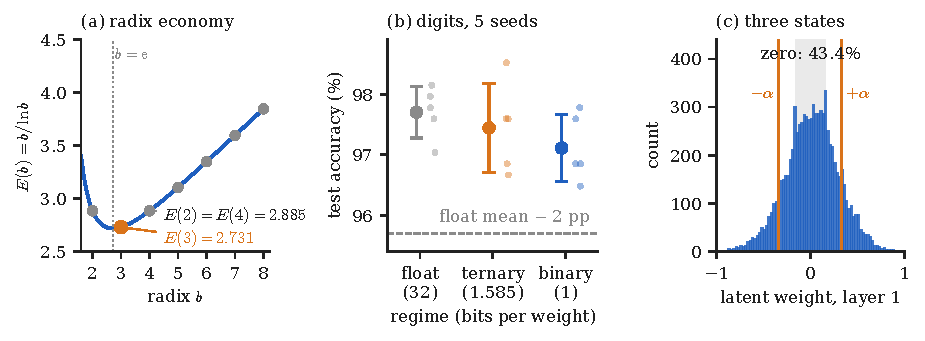
\includegraphics[width=\linewidth]{fig_algo.pdf}
\caption{(a) Radix economy $E(b)=b/\ln b$; integer radices in grey, $b=3$ in orange, the continuous optimum $b=\e$ dotted. (b) Digits test accuracy by weight regime: mean $\pm$ sd (large markers) and the five seeds (small markers); the dashed line marks $2$ percentage points below the float mean. (c) Latent layer-1 weights of the seed-0 ternary network: the grey band $|W|\le\Delta$ is the zero state (fraction $0.4343$ of this layer), and the orange lines mark $\pm\alpha$, the values assigned to the two signed states.}\label{fig:main}
\end{figure}

\section{Discussion: the triad in computation}\label{sec:triad}
\paragraph{The pair and its explicit zero.} A ternary weight is the triad $\{-s,0,s\}$ with $s=\alpha$: the pair $\pm\alpha$ carries excitation and inhibition, and $0$ is an explicit third state. A binary weight $\{-\alpha,+\alpha\}$ is the pair without its zero, so every connection must vote. The difference is exact under the involution $\iota(w)=-w$ \cite{SSynth}. The ternary quantiser is odd, $\alpha T_\Delta(-W)=-\alpha T_\Delta(W)$, and it sends the whole band $|W|\le\Delta$ to the fixed point $0$ of $\iota$. An odd map $Q$ into an alphabet $A=-A$ must satisfy $Q(0)=-Q(0)$, so $0\in A$; hence no odd quantiser onto $\{-\alpha,\alpha\}$ exists, and the convention $\sgn(0)=+1$ breaks the pair symmetry at one point. Balanced ternary shows that the triad is a complete arithmetic in its own right (\cref{thm:bt}): the width-$d$ range is $0$ plus $M_d$ pairs $\pm m$, negation is the pair exchange $s\leftrightarrow-s$, the sign sits in the leading trit, the carries stay in the triad, and rounding is truncation, that is, setting trits to the zero state. Negation $\iota(n)=-n$ is an instance of the involution of the synthesis paper \cite{SSynth}: its fixed set is $\{0\}$, and $n=\sgn(n)\,|n|$ is the product of a factor odd under $\iota$, the sign, which is the leading nonzero trit (\cref{thm:bt}d) and carries the direction, and a factor even under $\iota$, $|n|$, which carries the magnitude.

\paragraph{Three states are the economical radix.} Among integer numbers of states per digit, three uniquely minimises the growth rate $b/\ln b$ (\cref{prop:radix}); for the exact cost, three is a cheapest choice for every $N\ge2^{16}$ and the only cheapest choice for every $N\ge2^{27}$ (\cref{thm:eventual}). Three states are enough, and from $2^{27}$ on, fewer or more cost strictly more.

\paragraph{The thirds and the zero state.} Three exact instances of the thirds occur here. The zeros of one trit's generating function lie at $\frac13$ and $\frac23$ of a turn (\cref{prop:gf}). A probe reading one trit decoheres completely at $\frac13$ and $\frac23$ of its period (\cref{cor:probe}). And the least-squares ternary quantiser of uniformly distributed weights writes exactly $\frac23$ of them as $\pm\alpha$ and emits exactly $\frac13$ into the zero state (\cref{prop:lm}d). For other laws the emitted share is set by the law: $0.4595$ for Gaussian and $0.6321$ for Laplace weights at the optimum, and $0.35$, $0.4235$ and $0.5034$ under the $0.7$ rule (\cref{prop:lm}e); the trained networks emit $0.4325$. The emitted weights cost no arithmetic at inference, and the accuracy of \cref{tab:twn} is reached without them. Their positions are part of the stored model, and the entropy of $1.5527$ bits per weight counts them.

\paragraph{The observer and the next triad.} The comparator of two registers returns a trit (\cref{thm:bt}e), which can itself be a digit of a new register; a hidden unit reads a ternary-weighted sum, and its output enters the ternary rows of the next layer. In both cases the observer of one triad is a member of the next. This is the structure found in the balanced cortex, where each neuron reads a zero-sum ternary input and its output becomes an entry of other neurons' ternary rows \cite{SNeuro}, and in the probe of \cite{SQuant}, whose coherence reads a spin-1 triad (\cref{cor:probe}). The trained ternary networks also hold their two signed states in nearly equal shares ($0.3018$ and $0.2658$), close to the balanced pair.

\paragraph{The companion papers.} The connections are identities. The generating function $z^{-1}+1+z$ of one digit is the partition function of the uniform three-state spin, whose Lee--Yang zeros lie at $\frac13$ and $\frac23$ of a turn and which is the positive merge of two spin-$\frac12$ pairs at coupling $\frac12\ln2$ \cite{SMath,SQuant}. Evaluated at $z=\e^{-2i\lambda t}$ and divided by $3$, it is the coherence $(1+2\cos2\lambda t)/3$ of a probe qubit reading a maximally mixed spin-1 \cite{SQuant}, and a width-$d$ register read in the same way decoheres the probe at the $3^d$-ths of its period (\cref{cor:probe}). A ternary weight matrix has the alphabet of the ternary connectivity of the balanced cortex, whose rows take values in $\{+1,0,-J_X\}/\sqrt K$ \cite{SNeuro}; in a ternary-weight network the pair is symmetric, $\{+\alpha,0,-\alpha\}$.

\paragraph{Outlook.} \Cref{prop:lm}b gives the least-squares threshold $\Delta=\alpha/2$ for any weight law, so the next step is to train with the threshold set by the empirical law of each layer in place of the $0.7$ rule, and to carry the comparison of ternary, binary and float weights to larger networks and data sets.

\section{Data and sources}\label{sec:data}
\emph{Data set.} Optical Recognition of Handwritten Digits, E.~Alpaydin and C.~Kaynak (1998), University of California, Irvine \cite{uci_digits}: the test partition only, 1797 images of $8\times8$ integer pixel values $0$--$16$ (counts of on-pixels in nonoverlapping $4\times4$ blocks of $32\times32$ bitmaps written by 13 people), in 10 classes with $178,182,177,183,181,182,181,179,174,180$ images for the digits $0$ to $9$. We used all 1797 images, split 70/30 by class as described in \cref{sec:twn}; the 3823-image training partition of the same data set was not used.

\emph{External values quoted.} The cost model (product of radix and width) and the statements on Setun, negation and rounding are from Hayes~\cite{hayes2001}; the threshold factor $0.7$ and the approximate thresholds $\frac13a$ and $0.6\sigma$ are from \cite{twn2016}; Max's tabulated values $0.6120$, $1.2240$, $0.1902$ and $0.3634$ \cite{max1960} are used for comparison with the closed forms of \cref{prop:lm}.

\emph{Numerical inputs.} None besides the data set. The constants $\e$, $\ln2$, $\ln3$, $\phi$, $\Phi$ and $\mathrm{erf}$ enter through the closed forms stated, evaluated in double precision; $u^*$ is the root of $\phi(u)=2u(1-\Phi(u))$ found by bisection to $10^{-12}$. The finite-$N$ costs and the exceptional values of \cref{thm:eventual} are computed exactly in integer arithmetic; the balanced-ternary enumerations, the network results and the summary statistics are computed from the definitions and procedures stated in \cref{sec:radix,sec:bt,sec:twn}. The hyperparameters of \cref{sec:twn} and the threshold factor $0.7$ of \cite{twn2016} are fixed choices, not measured values.


\begin{thebibliography}{99}\small
\bibitem{hayes2001} B.~Hayes, Third base, \emph{American Scientist} \textbf{89}(6) (2001) 490, doi:10.1511/2001.40.3268.
\bibitem{knuth1997} D.~E.~Knuth, \emph{The Art of Computer Programming, Vol.~2: Seminumerical Algorithms}, 3rd ed., Addison-Wesley, Reading, MA, 1997, Section~4.1.
\bibitem{binaryconnect2015} M.~Courbariaux, Y.~Bengio, J.-P.~David, BinaryConnect: Training deep neural networks with binary weights during propagations, in \emph{Advances in Neural Information Processing Systems 28 (NIPS 2015)}, 2015, pp.~3123--3131; arXiv:1511.00363.
\bibitem{xnor2016} M.~Rastegari, V.~Ordonez, J.~Redmon, A.~Farhadi, XNOR-Net: ImageNet classification using binary convolutional neural networks, in \emph{Computer Vision -- ECCV 2016, Part IV}, Lecture Notes in Computer Science \textbf{9908}, Springer, 2016, pp.~525--542, doi:10.1007/978-3-319-46493-0\_32.
\bibitem{twn2016} F.~Li, B.~Zhang, B.~Liu, Ternary weight networks, arXiv:1605.04711v2 (2016).
\bibitem{bitnet158} S.~Ma, H.~Wang, L.~Ma, L.~Wang, W.~Wang, S.~Huang, L.~Dong, R.~Wang, J.~Xue, F.~Wei, The era of 1-bit LLMs: All large language models are in 1.58 bits, arXiv:2402.17764 (2024).
\bibitem{SMath} A.~Singh, Pair Balance and the Riemann Zeros: The Signed Current, the Mirror and the Merge, and the Prime Two, manuscript, 25 September 2026.
\bibitem{SQuant} A.~Singh, The Riemann Kernel as a Quantum State: Wigner Negativity, Decoherence at the Thirds and Lee--Yang Zeros, manuscript, 25 September 2026.
\bibitem{SNeuro} A.~Singh, The Balanced Pair in Excitable Tissue: What a Membrane Reading Determines, and the Balanced Cortex, manuscript, 25 September 2026.
\bibitem{SSynth} A.~Singh, What a Zero Is: One Involution across Mathematics, Physics, Chemistry, Neuroscience, Computation and the Giant Planets, manuscript, 25 September 2026.
\bibitem{max1960} J.~Max, Quantizing for minimum distortion, \emph{IRE Transactions on Information Theory} \textbf{6}(1) (1960) 7--12, doi:10.1109/TIT.1960.1057548.
\bibitem{uci_digits} E.~Alpaydin, C.~Kaynak, Optical Recognition of Handwritten Digits [data set], UCI Machine Learning Repository, 1998, doi:10.24432/C50P49, \url{https://archive.ics.uci.edu/dataset/80} (accessed 24 September 2026).
\bibitem{lloyd1982} S.~P.~Lloyd, Least squares quantization in PCM, \emph{IEEE Transactions on Information Theory} \textbf{28}(2) (1982) 129--137, doi:10.1109/TIT.1982.1056489.
\bibitem{adam} D.~P.~Kingma, J.~Ba, Adam: A method for stochastic optimization, in \emph{3rd International Conference on Learning Representations (ICLR 2015)}, San Diego, 2015; arXiv:1412.6980.
\bibitem{he2015} K.~He, X.~Zhang, S.~Ren, J.~Sun, Delving deep into rectifiers: Surpassing human-level performance on ImageNet classification, in \emph{2015 IEEE International Conference on Computer Vision (ICCV)}, 2015, pp.~1026--1034, doi:10.1109/ICCV.2015.123.
\end{thebibliography}
\end{document}
